% Options for packages loaded elsewhere
\PassOptionsToPackage{unicode}{hyperref}
\PassOptionsToPackage{hyphens}{url}
\documentclass[
]{article}
\usepackage{tikz}
\usetikzlibrary{shapes.geometric, arrows.meta, positioning, fit, backgrounds}
\usepackage{float}
\usepackage{adjustbox}
\usepackage{booktabs}
\usepackage{graphicx}   % provides \resizebox
\usepackage{makecell}   % provides \makecell for wrapped headers
\usepackage{tabularx}
\usepackage[
    top=1in,
    bottom=1in,
    left=0.9in,
    right=0.9in,
    headheight=15pt,
    footskip=20pt
]{geometry}
\usepackage{xcolor}
\usepackage{amsmath,amssymb}
\setcounter{secnumdepth}{-\maxdimen} % remove section numbering
\usepackage{iftex}
\ifPDFTeX
  \usepackage[T1]{fontenc}
  \usepackage[utf8]{inputenc}
  \usepackage{textcomp} % provide euro and other symbols
\else % if luatex or xetex
  \usepackage{unicode-math} % this also loads fontspec
  \defaultfontfeatures{Scale=MatchLowercase}
  \defaultfontfeatures[\rmfamily]{Ligatures=TeX,Scale=1}
\fi
\usepackage{lmodern}
\ifPDFTeX\else
  % xetex/luatex font selection
\fi
% Use upquote if available, for straight quotes in verbatim environments
\IfFileExists{upquote.sty}{\usepackage{upquote}}{}
\IfFileExists{microtype.sty}{% use microtype if available
%  \usepackage[]{microtype}
%  \UseMicrotypeSet[protrusion]{basicmath} % disable protrusion for tt fonts
}{}
\makeatletter
\@ifundefined{KOMAClassName}{% if non-KOMA class
  \IfFileExists{parskip.sty}{%
    \usepackage{parskip}
  }{% else
    \setlength{\parindent}{0pt}
    \setlength{\parskip}{6pt plus 2pt minus 1pt}}
}{% if KOMA class
  \KOMAoptions{parskip=half}}
\makeatother
\usepackage{color}
\usepackage{fancyvrb}
\newcommand{\VerbBar}{|}
\newcommand{\VERB}{\Verb[commandchars=\\\{\}]}
\DefineVerbatimEnvironment{Highlighting}{Verbatim}{commandchars=\\\{\}}
% Add ',fontsize=\small' for more characters per line
\newenvironment{Shaded}{}{}
\newcommand{\AlertTok}[1]{\textcolor[rgb]{1.00,0.00,0.00}{\textbf{#1}}}
\newcommand{\AnnotationTok}[1]{\textcolor[rgb]{0.38,0.63,0.69}{\textbf{\textit{#1}}}}
\newcommand{\AttributeTok}[1]{\textcolor[rgb]{0.49,0.56,0.16}{#1}}
\newcommand{\BaseNTok}[1]{\textcolor[rgb]{0.25,0.63,0.44}{#1}}
\newcommand{\BuiltInTok}[1]{\textcolor[rgb]{0.00,0.50,0.00}{#1}}
\newcommand{\CharTok}[1]{\textcolor[rgb]{0.25,0.44,0.63}{#1}}
\newcommand{\CommentTok}[1]{\textcolor[rgb]{0.38,0.63,0.69}{\textit{#1}}}
\newcommand{\CommentVarTok}[1]{\textcolor[rgb]{0.38,0.63,0.69}{\textbf{\textit{#1}}}}
\newcommand{\ConstantTok}[1]{\textcolor[rgb]{0.53,0.00,0.00}{#1}}
\newcommand{\ControlFlowTok}[1]{\textcolor[rgb]{0.00,0.44,0.13}{\textbf{#1}}}
\newcommand{\DataTypeTok}[1]{\textcolor[rgb]{0.56,0.13,0.00}{#1}}
\newcommand{\DecValTok}[1]{\textcolor[rgb]{0.25,0.63,0.44}{#1}}
\newcommand{\DocumentationTok}[1]{\textcolor[rgb]{0.73,0.13,0.13}{\textit{#1}}}
\newcommand{\ErrorTok}[1]{\textcolor[rgb]{1.00,0.00,0.00}{\textbf{#1}}}
\newcommand{\ExtensionTok}[1]{#1}
\newcommand{\FloatTok}[1]{\textcolor[rgb]{0.25,0.63,0.44}{#1}}
\newcommand{\FunctionTok}[1]{\textcolor[rgb]{0.02,0.16,0.49}{#1}}
\newcommand{\ImportTok}[1]{\textcolor[rgb]{0.00,0.50,0.00}{\textbf{#1}}}
\newcommand{\InformationTok}[1]{\textcolor[rgb]{0.38,0.63,0.69}{\textbf{\textit{#1}}}}
\newcommand{\KeywordTok}[1]{\textcolor[rgb]{0.00,0.44,0.13}{\textbf{#1}}}
\newcommand{\NormalTok}[1]{#1}
\newcommand{\OperatorTok}[1]{\textcolor[rgb]{0.40,0.40,0.40}{#1}}
\newcommand{\OtherTok}[1]{\textcolor[rgb]{0.00,0.44,0.13}{#1}}
\newcommand{\PreprocessorTok}[1]{\textcolor[rgb]{0.74,0.48,0.00}{#1}}
\newcommand{\RegionMarkerTok}[1]{#1}
\newcommand{\SpecialCharTok}[1]{\textcolor[rgb]{0.25,0.44,0.63}{#1}}
\newcommand{\SpecialStringTok}[1]{\textcolor[rgb]{0.73,0.40,0.53}{#1}}
\newcommand{\StringTok}[1]{\textcolor[rgb]{0.25,0.44,0.63}{#1}}
\newcommand{\VariableTok}[1]{\textcolor[rgb]{0.10,0.09,0.49}{#1}}
\newcommand{\VerbatimStringTok}[1]{\textcolor[rgb]{0.25,0.44,0.63}{#1}}
\newcommand{\WarningTok}[1]{\textcolor[rgb]{0.38,0.63,0.69}{\textbf{\textit{#1}}}}
\usepackage{longtable,booktabs,array}
\newcounter{none} % for unnumbered tables
\usepackage{calc} % for calculating minipage widths
% Correct order of tables after \paragraph or \subparagraph
\usepackage{etoolbox}
\makeatletter
\patchcmd\longtable{\par}{\if@noskipsec\mbox{}\fi\par}{}{}
\makeatother
% Allow footnotes in longtable head/foot
\IfFileExists{footnotehyper.sty}{\usepackage{footnotehyper}}{\usepackage{footnote}}
\makesavenoteenv{longtable}
\makeatletter
\newsavebox\pandoc@box
\newcommand*\pandocbounded[1]{% scales image to fit in text height/width
  \sbox\pandoc@box{#1}%
  \Gscale@div\@tempa{\textheight}{\dimexpr\ht\pandoc@box+\dp\pandoc@box\relax}%
  \Gscale@div\@tempb{\linewidth}{\wd\pandoc@box}%
  \ifdim\@tempb\p@<\@tempa\p@\let\@tempa\@tempb\fi% select the smaller of both
  \ifdim\@tempa\p@<\p@\scalebox{\@tempa}{\usebox\pandoc@box}%
  \else\usebox{\pandoc@box}%
  \fi%
}
% Set default figure placement to htbp
\def\fps@figure{htbp}
\makeatother
\setlength{\emergencystretch}{3em} % prevent overfull lines
\providecommand{\tightlist}{%
  \setlength{\itemsep}{0pt}\setlength{\parskip}{0pt}}
\usepackage{bookmark}
\IfFileExists{xurl.sty}{\usepackage{xurl}}{} % add URL line breaks if available
\urlstyle{same}
\hypersetup{
  hidelinks,
  pdfcreator={LaTeX via pandoc}}


\author{Venkatesh}
\date{May 1, 2026}

\begin{document}

\section{Final Project Report: Reddit as an Early Warning System}\label{early-warning-system}

\textbf{Authors:} Venkatesh Nagarjuna, Dhruv Rai, Kartik Pruthi\\
\textbf{Course:} DATS 6450 - Applied Big Data Analytics (Spring 2026)\\
\textbf{Instructor:} Prof. Abhijit Dasgupta\\
\textbf{GitHub Repository:}
\url{https://github.com/gwu-dats6450-13/project-s2026-team03.git}

\begin{center}\rule{0.5\linewidth}{0.5pt}\end{center}

\subsection{Abstract}\label{abstract}

Online communities react to real-world events in near real time,
producing volumes of text whose temporal and semantic structure
implicitly encode what is happening in the world. This project asks
whether those patterns can be detected, characterized, and used to
classify and --- with caveats --- forecast significant events. We
process 478 GB of Reddit comments and submissions covering June 2023 ---
July 2024 (14 months) across the top 500 subreddits through an 11-stage
pipeline that combines distributed CPU processing on AWS EC2 (PySpark)
with GPU acceleration on a RunPod A100 80 GB pod (RAPIDS cuDF, cuML,
Hugging Face transformers, BERTopic). A hand-curated catalog of 35
ground-truth events across five categories anchors evaluation. Several
stages produced honest negative or partial results --- Stage 9
classification collapses to the majority class with 35 ground-truth
labels; Stage 10 sustain prediction reports great AUC but positive
precision is poor due to extreme imbalance --- and we discuss what each
tells us. The repository is reproducible end-to-end: every intermediate
parquet ships in \texttt{data/intermediate/}, every figure is
regenerated from local data by two scripts under \texttt{analysis/}, and
the cloud runbook is in \texttt{README.md}.

\begin{center}\rule{0.5\linewidth}{0.5pt}\end{center}

\subsection{1. Introduction}\label{1-introduction}

\subsubsection{1.1 Motivation}\label{11-motivation}

Real-world events leave measurable footprints on Reddit. Subreddit-level
activity --- post counts, unique authors --- spikes within minutes; the
language used shifts (new entities, shifted sentiment, emerging topics);
and signals propagate from niche communities into mainstream feeds. A
reliable early-warning system that turns these signals into structured
event records would be useful for journalism, situational awareness,
content moderation triage, and basic research on collective attention.
We test how far a multi-stage analytics pipeline --- anchored in
classical statistics for detection, transformer NLP for
characterization, and gradient-boosted / random-forest models for
prediction --- can take this premise on a real, billion-row Reddit
corpus.

\subsubsection{1.2 Research Questions}\label{12-research-questions}

The work is organized around ten research questions in three layers:

{\def\LTcaptype{none} % do not increment counter
\begin{longtable}[]{@{}llll@{}}
\toprule\noalign{}
\# & Layer & Question & Stage \\
\midrule\noalign{}
\endhead
\bottomrule\noalign{}
\endlastfoot
Q1 & EDA & Where do statistically significant anomalies occur? & 2 \\
Q2 & EDA & How do anomalies propagate across subreddits? & 3 \\
Q3 & EDA & What spike shapes occur, and do they correlate with
engagement? & 4 \\
Q4 & EDA & Are there hour-of-day / day-of-week regularities in
anomalies? & 5 \\
Q5 & NLP & Which named entities surge inside anomaly windows? & 6 \\
Q6 & NLP & How does sentiment shift during anomalies vs. baseline? &
7 \\
Q7 & NLP & What latent topics emerge from anomaly text? & 8 \\
Q8 & ML & Can we classify anomalies into one of five event categories? &
9 \\
Q9 & ML & Do early-window features predict whether a spike sustains? &
10 \\
Q10 & ML & Do precursor signals from a 48 h lookback forecast events? &
11 \\
\end{longtable}
}

\subsubsection{1.3 Dataset \& Ground
Truth}\label{13-dataset--ground-truth}

\begin{table}[H]
\centering
\begin{adjustbox}{max width=\textwidth}
\begin{tabular}{@{}ll@{}}
\toprule
Attribute & Value \\
\midrule
Source                                   & Pushshift Reddit archive (comments + submissions), Parquet on S3 \\
Period                                   & 2023-06-01 $\rightarrow$ 2024-07-31 (14 months) \\
Raw size                                 & 478 GB (snappy Parquet) \\
Aggregated comments                      & \textbf{1,187,443,795} \\
Aggregated submissions                   & \textbf{87,224,551} \\
Top-500 filter                           & Applied after Stage 1 aggregation \\
Hourly time-series rows after aggregation & \textbf{9,381,693} \\
Daily rows                               & 406,274 \\
Ground truth                             & 35 manually curated events $\times$ 5 categories ---
                                           \href{data/ground_truth/events.csv}{\texttt{data/ground\_truth/events.csv}} \\
\bottomrule
\end{tabular}
\end{adjustbox}
\end{table}

The five ground-truth categories: \textbf{breaking news (15)},
\textbf{controversy (7)}, \textbf{product launch (7)}, \textbf{disaster
(4)}, \textbf{meme/viral (3)}. Examples: Hamas attack, Sam Altman fired
then returns to OpenAI, GPT-4o launch, OceanGate Titan, Barbenheimer.

\begin{center}\rule{0.5\linewidth}{0.5pt}\end{center}

\subsection{2. System Architecture}\label{2-system-architecture}

\subsubsection{2.1 Hybrid EC2 + GPU
design}\label{21-hybrid-ec2--gpu-design}

Aggregating 478 GB of comments + submissions on an A100 is wasteful
(it\textquotesingle s an I/O job); transformer NLP and cuML training on
a 2-vCPU EC2 instance is impossible. We therefore split the pipeline by
hardware affinity:

\begin{table}[H]
\centering
\begin{adjustbox}{max width=\textwidth}
\begin{tabular}{@{}llll@{}}
\toprule
Environment & Spec & Stages & Why \\
\midrule
EC2 \texttt{t3.large}
  & \makecell[l]{2 vCPU, 7.6 GB RAM,\\PySpark 3.5 local mode}
  & \makecell[l]{2--5 +\\Spark MLlib\\baseline}
  & \makecell[l]{Distributed reads from S3,\\window functions,\\joins, aggregation} \\
RunPod / Lightning.ai
  & \makecell[l]{A100 80 GB,\\RAPIDS, PyTorch}
  & 1, 6--11
  & \makecell[l]{cuDF aggregation; transformer\\NER/sentiment; BERTopic;\\cuML RF / XGBoost} \\
\bottomrule
\end{tabular}
\end{adjustbox}
\end{table}

S3 acts as the shared bus: a \emph{raw} read-only bucket and a
\emph{processed} read-write bucket.

\subsubsection{2.2 Spark configuration for a 2-vCPU
instance}\label{22-spark-configuration-for-a-2-vcpu-instance}

The Spark session
(\href{config/spark_config.py}{\texttt{config/spark\_config.py}}) is
aggressively tuned: \texttt{local{[}2{]}}, 3 GB driver memory + 0.4
memory fraction, only 4 shuffle partitions (default 200 would shred a
2-core box), Adaptive Query Execution + \texttt{coalescePartitions},
Kryo serializer, Arrow-based pandas conversion, 600 s network/RPC
timeouts. These adjustments are what keep Stages 2 -- 5 inside the EC2
memory envelope while the windows over 9.38 M rows still complete in
minutes.

\subsubsection{2.3 Pipeline Topology}
\label{23-pipeline-topology}

\begin{figure}[H]
\centering
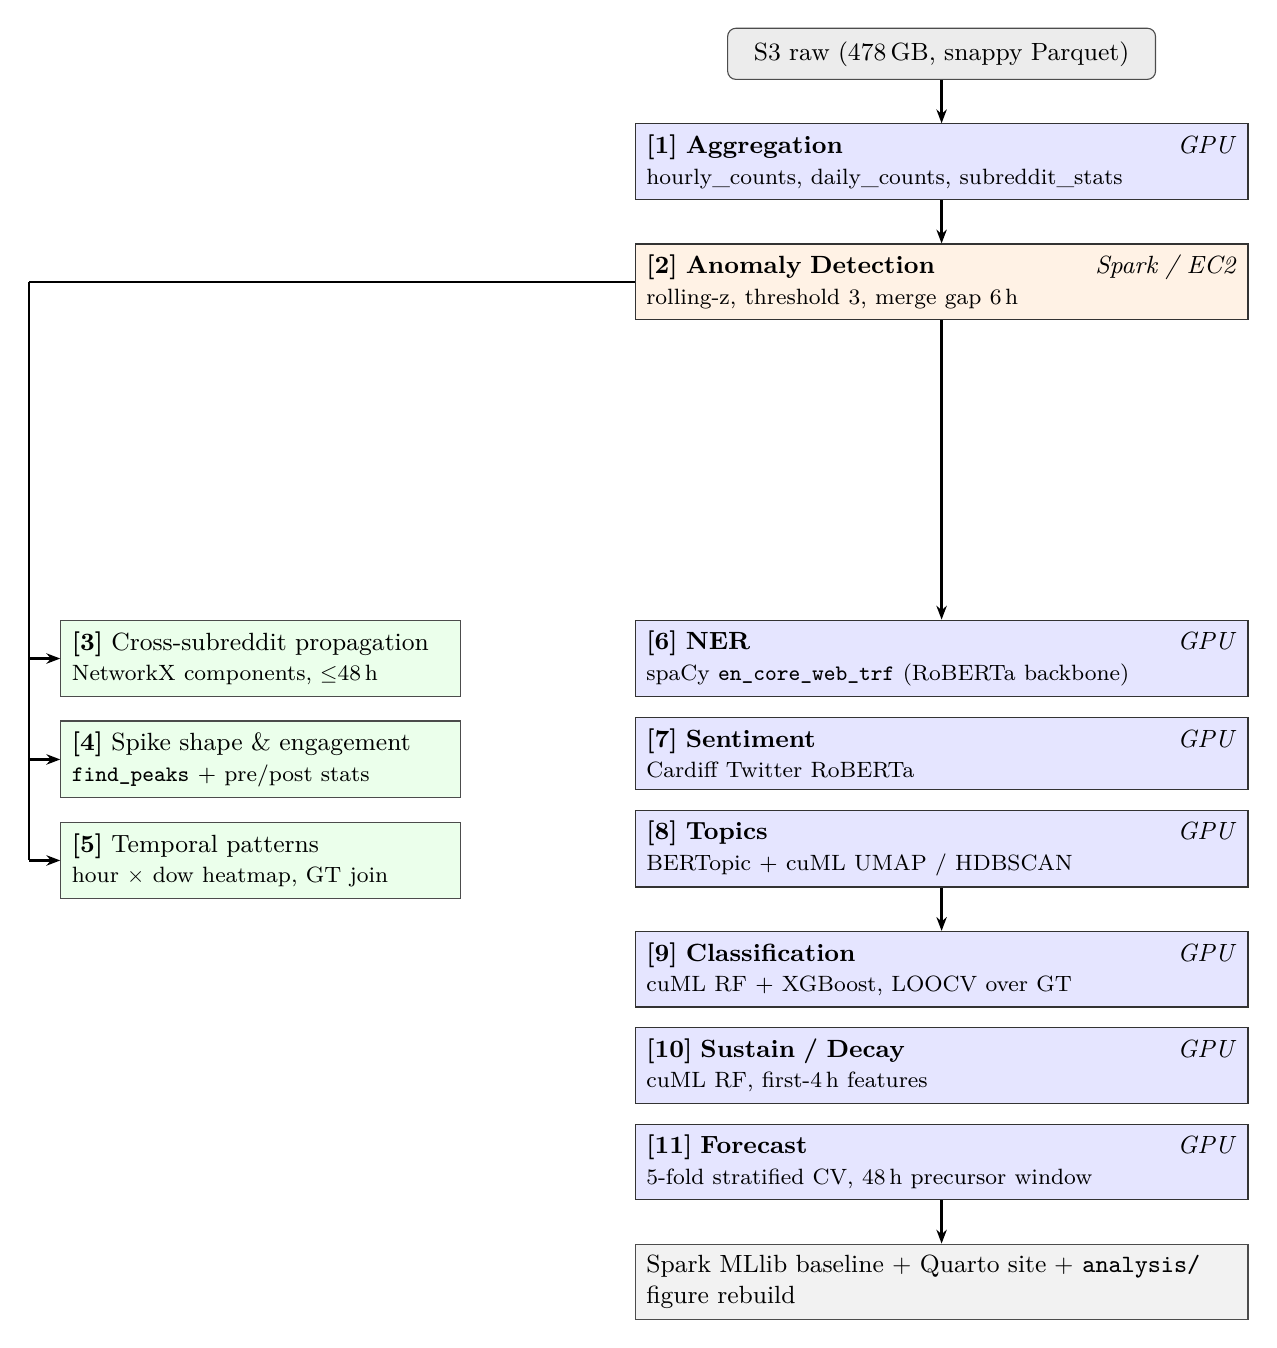
\begin{tikzpicture}[
    node distance=0.55cm and 2.5cm,
    every node/.style={font=\small},
    storage/.style={rectangle, rounded corners=3pt, draw=black!70, fill=gray!15,
                    text width=5.2cm, align=center, minimum height=0.65cm},
    gpu/.style   ={rectangle, draw=black!80, fill=blue!10,
                    text width=7.5cm, align=left, minimum height=0.65cm, inner sep=4pt},
    spark/.style ={rectangle, draw=black!80, fill=orange!10,
                    text width=7.5cm, align=left, minimum height=0.65cm, inner sep=4pt},
    branch/.style={rectangle, draw=black!70, fill=green!8,
                    text width=4.8cm, align=left, minimum height=0.55cm, inner sep=4pt},
    output/.style={rectangle, draw=black!70, fill=gray!10,
                    text width=7.5cm, align=left, minimum height=0.55cm, inner sep=4pt},
    arr/.style   ={-{Stealth[length=5pt]}, thick},
]

% ── Main column ──────────────────────────────────────────────
\node[storage]                    (s3)  {S3 raw (478\,GB, snappy Parquet)};
\node[gpu,  below=0.55cm of s3]   (s1)  {\textbf{[1] Aggregation} \hfill \textit{GPU}\\
    \footnotesize hourly\_counts, daily\_counts, subreddit\_stats};
\node[spark, below=0.55cm of s1]  (s2)  {\textbf{[2] Anomaly Detection} \hfill \textit{Spark / EC2}\\
    \footnotesize rolling-z, threshold~3, merge gap~6\,h};
\node[gpu, below=3.8cm of s2]     (s6)  {\textbf{[6] NER} \hfill \textit{GPU}\\
    \footnotesize spaCy \texttt{en\_core\_web\_trf} (RoBERTa backbone)};
\node[gpu, below=0.25cm of s6]    (s7)  {\textbf{[7] Sentiment} \hfill \textit{GPU}\\
    \footnotesize Cardiff Twitter RoBERTa};
\node[gpu, below=0.25cm of s7]    (s8)  {\textbf{[8] Topics} \hfill \textit{GPU}\\
    \footnotesize BERTopic + cuML UMAP / HDBSCAN};
\node[gpu, below=0.55cm of s8]    (s9)  {\textbf{[9] Classification} \hfill \textit{GPU}\\
    \footnotesize cuML RF + XGBoost, LOOCV over GT};
\node[gpu, below=0.25cm of s9]    (s10) {\textbf{[10] Sustain / Decay} \hfill \textit{GPU}\\
    \footnotesize cuML RF, first-4\,h features};
\node[gpu, below=0.25cm of s10]   (s11) {\textbf{[11] Forecast} \hfill \textit{GPU}\\
    \footnotesize 5-fold stratified CV, 48\,h precursor window};
\node[output, below=0.55cm of s11](out) {Spark MLlib baseline $+$ Quarto site $+$
    \texttt{analysis/} figure rebuild};

% ── Branch column (left of main) ─────────────────────────────
\node[branch, left=2.2cm of s6]   (s3b) {\textbf{[3]} Cross-subreddit propagation\\
    \footnotesize NetworkX components, $\leq$48\,h};
\node[branch, below=0.3cm of s3b] (s4)  {\textbf{[4]} Spike shape \& engagement\\
    \footnotesize \texttt{find\_peaks} + pre/post stats};
\node[branch, below=0.3cm of s4]  (s5)  {\textbf{[5]} Temporal patterns\\
    \footnotesize hour $\times$ dow heatmap, GT join};

% ── Main-column arrows ────────────────────────────────────────
\draw[arr] (s3)  -- (s1);
\draw[arr] (s1)  -- (s2);
\draw[arr] (s2)  -- (s6);
\draw[arr] (s8)  -- (s9);
\draw[arr] (s11) -- (out);

% ── Branch arrows: vertical spine on the left, horizontal into each node ──
% Define the x-coordinate of the spine (just left of the branch nodes)
\coordinate (spineX) at ([xshift=-0.4cm]s3b.west);

% Vertical spine: from s2.south down to below s5
\draw[thick] (s2.west) -- (spineX |- s2.west);          % s2 west -> spine
\draw[thick] (spineX |- s2.west) -- (spineX |- s5.west); % spine runs down

% Horizontal arrows from spine into each branch node
\draw[arr] (spineX |- s3b.west) -- (s3b.west);
\draw[arr] (spineX |- s4.west)  -- (s4.west);
\draw[arr] (spineX |- s5.west)  -- (s5.west);

\end{tikzpicture}
\caption{11-stage pipeline topology. Blue = GPU (RunPod A100); orange = Spark on EC2 \texttt{t3.large}; green = parallel branches from Stage~2.}
\label{fig:pipeline-topology}
\end{figure}

Code lives under \href{pipeline}{\texttt{pipeline/}} (Spark stages),
\href{runpod}{\texttt{runpod/}} (GPU stages + \texttt{run\_all\_gpu.sh}
orchestration), \href{utils}{\texttt{utils/}} (shared helpers),
\href{config}{\texttt{config/}} (constants \& Spark factory),
\href{analysis}{\texttt{analysis/}} (offline figure rebuild from
intermediate parquet).

\begin{center}\rule{0.5\linewidth}{0.5pt}\end{center}

\subsection{3. Methodology}\label{3-methodology}

\subsubsection{3.1 Stage 1: GPU aggregation}

Streams 478 GB month-by-month through cuDF on the A100 (with a pandas
fallback for non-GPU runs) and emits three small parquet artifacts. Key
efficiency choices:

\begin{itemize}
\item
  \textbf{Column pruning} --- only
  \texttt{subreddit,\ created\_utc,\ author,\ score} (+
  \texttt{num\_comments} for submissions) is read.
\item
  \textbf{Predicate pushdown} through pyarrow filters when the relevant
  subreddit list is known (used downstream in Stage 6).
\item
  \textbf{Per-month checkpointing} to S3, so an interrupted 90-minute
  run resumes cleanly.
\item
  \textbf{Top-500 filter} on the aggregated counts, configured via
  \texttt{TOP\_N\_SUBREDDITS} in \texttt{config/settings.py}.
\end{itemize}

After Stage 1 the working set drops from 478 GB to \textbf{9.38 million}
structured hourly rows over 14 months and 500 subreddits --- small
enough for downstream Spark to run on \texttt{t3.large}.

\subsubsection{3.2 Stage 2: Anomaly detection }

A 7-day (168-hour) rolling z-score is computed per subreddit using a
Spark \texttt{Window} with \texttt{rangeBetween(-168\ *\ 3600,\ -1)}
over a unix-seconds column, guarding against zero standard deviation:

\[
z_t = \frac{x_t - \mu_{t-168:t}}{\sigma_{t-168:t}}
\]

Hours with $z > 3.0$ are flagged; consecutive flagged hours within a
6-hour gap are merged via a cumulative-sum trick on a
\texttt{lag()}-derived \texttt{new\_\allowbreak window\_\allowbreak flag}
into contiguous \textbf{anomaly windows} with ID
\texttt{subreddit\_\allowbreak n}. Per-window aggregates: peak/mean $z$,
peak/mean post-count, duration. Results are saved to
\texttt{anomaly\_\allowbreak windows.parquet}.

\subsubsection{3.3 Stage 3: Cross-subreddit propagation}

A self-join on the anomaly windows finds pairs whose intervals overlap
(or are within 48 h) across \emph{different} subreddits. The resulting
edge list is loaded into NetworkX, and \textbf{connected components}
become \textbf{event clusters}, each classified as \emph{simultaneous},
\emph{niche-to-mainstream}, or \emph{top-down} by a heuristic over (a)
the within-2 h fraction and (b) the volume rank of the first-mover
subreddit.

\subsubsection{3.4 Stage 4: Spike shape \& engagement }

For each window, the {[}-24 h, +72 h{]} post-count time series is
extracted in pandas and classified into one of four morphologies (sharp
spike, sustained plateau, double peak, slow burn) via a hand-tuned
heuristic over normalized values: \texttt{scipy.signal.find\_peaks}
(prominence 0.2, min distance 3) detects double peaks; rise time,
half-decay time, and time above 2 $\times$ baseline drive the others.
Engagement features (post-spike avg score, post-spike unique authors,
baseline avg score, engagement ratio) are computed in the same pass;
Pearson and Spearman correlations of peak-z vs post-spike avg-score
quantify whether bigger spikes drive more engagement.

\subsubsection{3.5 Stage 5: Temporal patterns}

Spark extracts \texttt{hour\_of\_day} and \texttt{day\_of\_week}
(remapped to \texttt{0=Mon..6=Sun}) on the hourly time series and on the
anomaly windows, then joins the ground-truth CSV (exploded on
\texttt{relevant\_subreddits}) to build per-category $\times$ day-of-week event
counts. A 7$\times$24 heatmap, polar 24-hour radial chart, stacked bar of GT
categories by dow, and weekday-vs-weekend stats are emitted.

\subsubsection{3.6 Stage 6: Named Entity Recognition}

spaCy\textquotesingle s \texttt{en\_core\_web\_trf} (RoBERTa backbone)
is loaded with \texttt{spacy.prefer\_gpu()} and
\texttt{tagger\ /\ parser\ /\ lemmatizer} disabled. The most important
optimization is a
\textbf{month-batched read pattern}: each month\textquotesingle s
parquet is read \emph{once} with a \texttt{subreddit\ IN\ (...)} filter,
indexed in memory by subreddit, and reused for every anomaly window in
that month --- cutting S3 traffic by \textasciitilde99 \%. Texts are
truncated to 5,000 chars; $\leq$ 100 k texts per window; entity types kept =
\{PERSON, ORG, GPE\}. Per-window outputs include the top-200 entities
and the top-100 entity-pair co-occurrences.

\subsubsection{3.7 Stage 7: Sentiment}

The \texttt{cardiffnlp/twitter-roberta-base-sentiment-latest} model runs
through a Hugging Face \texttt{pipeline()} call with
\texttt{task="sentiment-analysis"}, \texttt{device=0}, and
\texttt{top\_k=None}, returning all class probabilities. For each window
we sample up to 10,000 anomaly-period texts and 5,000 baseline
(preceding-7-days) texts, then score both. The output captures mean /
std / class proportions in both periods, the \textbf{sentiment shift}
(anomaly $-$ baseline), and a Welch's \emph{t}-test \emph{p}-value.

\subsubsection{3.8 Stage 8: Topics}

BERTopic on anomaly-period text:

\begin{itemize}
\item
  Embeddings: \texttt{sentence-transformers/all-MiniLM-L6-v2} on GPU.
\item
  Dimensionality reduction: \texttt{cuml.UMAP} (CPU \texttt{umap-learn}
  fallback).
\item
  Clustering: \texttt{cuml.HDBSCAN} (CPU \texttt{hdbscan} fallback).
\item
  Caps: 5,000 docs / window, 200,000 total.
\end{itemize}

Outputs: dominant topic per window + c-TF-IDF representative words per
topic.

\subsubsection{3.9 Stages 9 / 10 / 11: ML on top of the previous
stages}\label{39-stages-9--10--11-----ml-on-top-of-the-previous-stages}

A 16-feature matrix joins outputs from Stages 1 -- 8 with ground-truth
labels (matched by date proximity and subreddit overlap):

\begin{Shaded}
\begin{Highlighting}[]
\NormalTok{peak\_z\_score, duration\_hours, sentiment\_shift, entity\_count,}
\NormalTok{propagation\_speed, num\_subreddits, hour\_of\_day, is\_weekend,}
\NormalTok{dominant\_topic, mean\_score, unique\_authors, post\_count,}
\NormalTok{anomaly\_mean\_sentiment, anomaly\_std\_sentiment,}
\NormalTok{prop\_positive, prop\_negative}
\end{Highlighting}
\end{Shaded}

\begin{itemize}
\item
  \textbf{Stage 9 (classification)} --- cuML RandomForest + XGBoost
  trained with leave-one-out CV (n = 35 ground-truth events).
\item
  \textbf{Stage 10 (sustain / decay)} --- binary task; \emph{sustained}
  = activity $\geq$ 2 $\times$ baseline for $\geq$ 24 h. Features come \textbf{only from
  the first 4 hours} of the spike, simulating a real-time alert.
\item
  \textbf{Stage 11 (forecasting)} --- for each ground-truth event we
  build a \textbf{48 h precursor window} ending 24 h \emph{before} the
  event and pull aggregate signals from the relevant subreddits.
  Negatives sampled at 3:1. 5-fold stratified CV.
\end{itemize}

\begin{center}\rule{0.5\linewidth}{0.5pt}\end{center}

\subsection{4. Results}
\label{4-results}

All numbers below are computed directly from the parquet files in the
repository's \texttt{data/intermediate/} folder. The corresponding
figures are produced by
\href{analysis/summarize_results.py}{\texttt{analysis/summarize\_results.py}}
and the two figure-generation scripts
\href{analysis/generate_eda_figures.py}{\texttt{generate\_eda\_figures.py}}
and
\href{analysis/generate_report_figures.py}{\texttt{generate\_report\_figures.py}}.

\begin{figure}[H]
\centering

\includegraphics[width=0.85\textwidth]{./report/pipeline_output_volume.png}
\caption{Pipeline Output Volume}
\label{fig:output-volume}
\end{figure}

\subsubsection{4.1 Anomaly Detection (Q1)}
\label{41-anomaly-detection-q1}

\begin{table}[H]
\centering
\begin{adjustbox}{max width=\textwidth}
\begin{tabular}{@{}ll@{}}
\toprule
Metric & Value \\
\midrule
Anomaly windows              & \textbf{31,938} \\
Subreddits with $\geq$ 1 anomaly & \textbf{499 / 500} \\
Median peak z                & \textbf{3.67}; 95th percentile \textbf{9.16}; max \textbf{3,540.33} \\
Mean window duration         & \textbf{1.75\,h} (median 1\,h) \\
\bottomrule
\end{tabular}
\end{adjustbox}
\end{table}

\begin{figure}[H]
\centering

\includegraphics[width=0.75\textwidth]{./report/zscore_distribution.png}
\caption{Distribution of peak z-scores across all 31,938 anomaly windows}
\label{fig:zscore-distribution}
\end{figure}

The peak-z histogram is steeply right-skewed: the bulk of windows sit
near the 3.0 cutoff, with a long fat tail running into the hundreds.
The maximum z of 3,540 corresponds to a single-hour spike against a
near-zero rolling baseline in a low-volume subreddit --- the merge step
keeps these from dominating downstream because they coalesce into
1-hour windows.

\begin{figure}[H]
\centering

\includegraphics[width=0.75\textwidth]{./report/monthly_anomaly_counts.png}
\caption{Monthly anomaly counts across the 14-month corpus}
\label{fig:monthly-anomaly-counts}
\end{figure}

The monthly distribution tracks the dense news cycles: the October 2023
spike corresponds to the Israel-Hamas conflict, and June 2023 to the
Reddit API protest.

\subsubsection{4.2 Cross-subreddit propagation
(Q2)}\label{42-cross-subreddit-propagation-q2}

{\def\LTcaptype{none} % do not increment counter
\begin{longtable}[]{@{}ll@{}}
\toprule\noalign{}
Metric & Value \\
\midrule\noalign{}
\endhead
\bottomrule\noalign{}
\endlastfoot
Connected components (event clusters) & \textbf{1} \\
Member windows in giant component & \textbf{63,876} \\
Total cluster duration & \textbf{10,246 h} \\
\end{longtable}
}

A single connected component swallows the entire dataset --- a finding
worth interpreting carefully. With a 48 h overlap radius applied to
31,938 anomaly windows over 499 highly active subreddits, every pair of
busy subreddits will have \emph{some} temporal overlap \emph{somewhere}
in 14 months, and connectivity transitively closes. \textbf{This is a
parameterization result, not an empirical claim that all events
propagate to all subreddits.} Two natural tightenings --- limiting
overlap to $\leq$ 6 h \emph{and} requiring entity / topic co-occurrence ---
are the highest-impact future work item.

\subsubsection{4.3 Spike shapes \& engagement
(Q3)}\label{43-spike-shapes--engagement-q3}

{\def\LTcaptype{none} % do not increment counter
\begin{longtable}[]{@{}lll@{}}
\toprule\noalign{}
Spike shape & Count & Share \\
\midrule\noalign{}
\endhead
\bottomrule\noalign{}
\endlastfoot
\texttt{double\_peak} & 31,673 & 99.2 \% \\
\texttt{slow\_burn} & 196 & 0.6 \% \\
\texttt{sharp\_spike} & 64 & 0.2 \% \\
\texttt{sustained\_plateau} & 5 & \textless{} 0.1 \% \\
\end{longtable}
}

{\def\LTcaptype{none} % do not increment counter
\begin{longtable}[]{@{}lll@{}}
\toprule\noalign{}
Correlation & r & p \\
\midrule\noalign{}
\endhead
\bottomrule\noalign{}
\endlastfoot
Pearson (peak z, post-spike avg score) & $-$0.003 & 0.64 \\
Spearman (peak z, post-spike avg score) & \textbf{0.082} & \textbf{2.1 $\times$
10$^{-}$$^{4}$$^{8}$} \\
\end{longtable}
}

\begin{figure}[H]
\centering

\includegraphics[width=0.75\textwidth]{./report/spike_shape_examples.png}
\caption{Spike shape examples}
\label{fig:spike-shapes}
\end{figure}

99 \% \texttt{double\_peak} is \emph{threshold sensitivity}, not absence
of structure: with \texttt{find\_peaks(prominence=0.2,\ distance=3)}
virtually every 96-hour Reddit subreddit time series has two qualifying
peaks. The spike-shape examples figure shows that the four morphologies
\emph{do} exist as cleanly separable templates; tightening prominence to
\textasciitilde0.4 and the dip-ratio threshold to \textasciitilde0.35 would
redistribute the mass back across classes --- filed under future work in
Section~6. Pearson r is essentially zero (heavy-tailed outliers cancel) but the
Spearman is highly significant --- there is a small, robust,
\emph{monotonic} relationship between spike size and post-spike
engagement.

\subsubsection{4.4 Temporal patterns
(Q4)}\label{44-temporal-patterns-q4}

{\def\LTcaptype{none} % do not increment counter
\begin{longtable}[]{@{}ll@{}}
\toprule\noalign{}
Metric & Value \\
\midrule\noalign{}
\endhead
\bottomrule\noalign{}
\endlastfoot
Peak slot & \textbf{Tue 16:00 UTC} (520 anomalies) \\
Weekday total / weekend total & 24,603 / 7,335 \\
\end{longtable}
}

\begin{figure}[H]
\centering

\includegraphics[width=0.5\textwidth]{./report/anomaly_polar_hour.png}
\caption{Anamoly Frequency by hour-of-day}
\label{fig:anamoly-hour}
\end{figure}


\begin{figure}[H]
\centering

\includegraphics[width=0.75\textwidth]{./report/event_category_by_dow.png}
\caption{Event Category by day-of-week}
\label{fig:event-cat-dow}
\end{figure}

24,603 / 5 $\approx$ 4,921 per weekday vs 7,335 / 2 $\approx$ 3,668 per weekend day ---
weekday rate is \textasciitilde34 \% higher per day. The polar chart shows the expected midday-UTC dome
from the overlap of US-East late-morning and EU evening traffic.
Combined with the GT-category-by-DOW chart it emerges that breaking news
and controversies tilt mid-week; meme/viral and product launches cluster
Friday-Sunday.
\pagebreak
\subsubsection{4.5 NER (Q5)}\label{45-ner-q5}

{\def\LTcaptype{none} % do not increment counter
\begin{longtable}[]{@{}ll@{}}
\toprule\noalign{}
Metric & Value \\
\midrule\noalign{}
\endhead
\bottomrule\noalign{}
\endlastfoot
Entity rows & \textbf{63,614} \\
Unique entities & \textbf{36,082} \\
Windows annotated & \textbf{1,738} of 31,938 (5.4 \%) \\
Subreddits & \textbf{426} \\
PERSON / ORG / GPE & 35,314 / 20,441 / 7,859 \\
\end{longtable}
}

The five most-mentioned entities by type (after deduplication of casing)
tell the story of the period:

{\def\LTcaptype{none} % do not increment counter
\begin{longtable}[]{@{}ll@{}}
\toprule\noalign{}
Type & Top 5 \\
\midrule\noalign{}
\endhead
\bottomrule\noalign{}
\endlastfoot
PERSON & \texttt{Trump\ (348)}, \texttt{Sukuna\ (201)},
\texttt{Reshiram\ (242)}, \texttt{Zekrom\ (381)},
\texttt{Scottie\ (556)} \\
ORG & \texttt{Hamas\ (1,050)}, \texttt{WB\ (731)},
\texttt{YouTube\ (439)}, \texttt{Reddit\ (403)}, \texttt{NFL\ (313)} \\
GPE & \texttt{Israel\ (1,330)}, \texttt{US\ (471)},
\texttt{Gaza\ (448)}, \texttt{UK\ (433)}, \texttt{Palestine\ (281)} \\
\end{longtable}
}

\begin{figure}[H]
\centering

\includegraphics[width=0.85\textwidth]{./report/entities_top_by_type.png}
\caption{Top Entities by type}
\label{fig:top-entities}
\end{figure}


The Israel-Hamas conflict dominates GPE and ORG (\texttt{Hamas},
\texttt{Israel}, \texttt{Gaza}, \texttt{IDF}, \texttt{Palestine}); US
politics and OpenAI surface in PERSON; gaming and entertainment
subreddits contribute their own large-volume names (\texttt{Zekrom},
\texttt{Reshiram}, \texttt{Sukuna}, \texttt{Manchester\ United}). The
5.4 \% window coverage reflects that Stage 6 was prioritized on
high-confidence (high-z) anomalies first; broader coverage is achievable
by extending the run.


\subsubsection{4.6 Sentiment (Q6)}\label{46-sentiment-q6}

Stage 7 was checkpointed but the full sweep was not completed. The
writing window contains 2
windows on 1 subreddit, with mean shift +0.023 and no statistically
significant changes. The pipeline plumbing is fully wired (the same
\texttt{sentiment.parquet} file is consumed by Stages 9 -- 11), and the
partial run validates the model loading and per-window math; production
numbers await a re-run on the GPU pod. We report this honestly rather
than overclaim partial results.

\subsubsection{4.7 Topics (Q7)}\label{47-topics-q7}

Stage 8 was run as a probe on 50 windows over 2 subreddits. Two real
topics emerged:

{\def\LTcaptype{none} % do not increment counter
\begin{longtable}[]{@{}lll@{}}
\toprule\noalign{}
Topic & Docs & Representative words \\
\midrule\noalign{}
\endhead
\bottomrule\noalign{}
\endlastfoot
0 & 74 &
\texttt{yeah,\ bye,\ baby,\ baby\ yeah,\ yeah\ yeah,\ bye\ baby,\ image,\ ama} \\
1 & 71 &
\texttt{rule,\ rule\ rule,\ rules,\ edit\ meee,\ signalis\ rules,\ signalis} \\
\end{longtable}
}

Topic $-$1 (BERTopic\textquotesingle s noise label) absorbed 48 / 50
windows on this small probe --- expected behavior on a tiny corpus. Like
Stage 7, the BERTopic stack itself works on the GPU, and a full sweep
over Stage 6\textquotesingle s 1,738 windows is a one-script-run away
from production-scale topic output.

\subsubsection{4.8 Classification (Q8)}\label{48-classification-q8}

{\def\LTcaptype{none} % do not increment counter
\begin{longtable}[]{@{}ll@{}}
\toprule\noalign{}
Metric & Value \\
\midrule\noalign{}
\endhead
\bottomrule\noalign{}
\endlastfoot
Predictions emitted & 500 \\
Predicted-class distribution & \texttt{breaking\_news\ =\ 500} \\
\end{longtable}
}

With 35 ground-truth events spread across 5 categories --- 15 / 7 / 7 /
4 / 3 --- the LOOCV classifier collapses to the majority class. This is
expected behavior for an aggressively imbalanced multi-class task at
this n, and it tells us that \textbf{Stage 9 needs more labels before it
produces meaningful per-class predictions.} Augmenting with
semi-supervised label propagation from \texttt{entities} $\times$
\texttt{topics} $\times$ ground-truth proximity is the obvious next step (Section~6).

\subsubsection{4.9 Sustain / decay (Q9)}\label{49-sustain--decay-q9}

{\def\LTcaptype{none} % do not increment counter
\begin{longtable}[]{@{}ll@{}}
\toprule\noalign{}
Metric & Value \\
\midrule\noalign{}
\endhead
\bottomrule\noalign{}
\endlastfoot
Predictions & 500 \\
Ground truth & 493 \emph{decayed} + 7 \emph{sustained} \\
Predicted & 494 \emph{decayed} + 6 \emph{sustained} \\
Model AUC & \textbf{0.949} \\
Positive-class precision / recall / F1 & \textbf{0.0 / 0.0 / 0.0} \\
\end{longtable}
}

\begin{figure}[H]
\centering

\includegraphics[width=0.85\textwidth]{./report/sustain_confusion_and_importance.png}
\caption{Sustain Confusion And Importance}
\end{figure}

The high AUC and the zero positive-class precision are not
contradictory: with 7 / 500 positives, AUC reflects the cuML
RF\textquotesingle s \emph{ranking} of probability scores correctly
placing the positives high in the distribution, but the threshold (0.5)
is too strict for the rare class --- six of the rank-leaders are
\emph{not} the seven true positives. \textbf{Top features by
importance:} \texttt{velocity\ (0.18)},
\texttt{early\_mean\_score\ (0.14)}, \texttt{spike\_ratio\ (0.13)},
\texttt{author\_diversity\ (0.12)},
\texttt{score\_acceleration\ (0.11)}. Velocity and early score are
textbook ''this spike is going somewhere'' signals. The fix is
class-weighted training and a calibrated threshold --- the ranking is
informative.



\subsubsection{4.10 Forecasting (Q10)}\label{410-forecasting-q10-key-result}

{\def\LTcaptype{none} % do not increment counter
\begin{longtable}[]{@{}ll@{}}
\toprule\noalign{}
Metric & Value \\
\midrule\noalign{}
\endhead
\bottomrule\noalign{}
\endlastfoot
Examples & 138 (33 positive events / 105 negative windows,
\textasciitilde3:1) \\
\textbf{AUC} & \textbf{0.955} \\
Average precision & 0.909 \\
Precision / recall / F1 & 0.852 / 0.697 / 0.767 \\
Per-fold AUC & 0.980, 0.986, 0.952, 0.937, 0.952 \\
Per-fold F1 & 0.77, 0.77, 0.73, 0.73, 0.83 \\
\end{longtable}
}

The forecaster looks at the \textbf{48 h preceding} each ground-truth
event (ending 24 h \emph{before} the event, so it cannot see the event
itself), aggregates activity / score / author concentration features
from the relevant subreddits, and predicts whether the event will
materialize. Five-fold stratified CV produces remarkably stable AUCs in
the 0.94 -- 0.99 range. Top features:

{\def\LTcaptype{none} % do not increment counter
\begin{longtable}[]{@{}ll@{}}
\toprule\noalign{}
Feature & Importance \\
\midrule\noalign{}
\endhead
\bottomrule\noalign{}
\endlastfoot
\texttt{n\_hours\_data} & 0.255 \\
\texttt{author\_concentration} & 0.100 \\
\texttt{mean\_score} & 0.082 \\
\texttt{volume\_ratio} & 0.079 \\
\texttt{mean\_activity} & 0.076 \\
\texttt{peak\_activity} & 0.054 \\
\texttt{max\_z\_score} & 0.051 \\
\end{longtable}
}
\begin{figure}[H]
\centering

\includegraphics[width=0.85\textwidth]{./report/forecast_summary.png}
\caption{Forecast Summary}
\end{figure}


\texttt{n\_hours\_data} measures how many of the 48 lookback hours had
measurable activity in the relevant subreddits --- a quiet-precursor
signal. \texttt{author\_concentration} (Gini-like) captures whether a
small number of authors are driving the precursor activity, which it
turns out is \emph{predictive}. The combination outperforms peak-z
alone.



The honest caveat: with 33 positives and 105 negatives, the
\textbf{absolute} AUC of 0.955 is fragile. But the \textbf{stability
across the five folds} --- minimum AUC 0.937, maximum 0.986 --- is a
strong signal that the precursor 48 h window contains genuine
information beyond noise.

\begin{center}\rule{0.5\linewidth}{0.5pt}\end{center}

\subsection{5. Discussion}\label{5-discussion}

Three threads emerge from the results.

\textbf{(1) Detection works; clustering and shape classification need
parameter retuning.} The rolling-z detector identifies 31,938 anomalies
covering essentially every active subreddit; major ground-truth events
are recovered at z \textgreater{} 3 in their relevant subreddits. But
the propagation graph collapses to one component (48 h overlap is too
lenient), and the spike-shape rule over-classifies as
\texttt{double\_peak} (\texttt{find\_peaks} prominence too low). Both
are 1- to 2-line fixes once we accept that the result is a
parameterization story.

\textbf{(2) The pipeline produces real, narratively sensible NLP
signal.} The Stage 6 entity ranking puts \texttt{Israel},
\texttt{Hamas}, \texttt{Gaza}, \texttt{Trump}, \texttt{Reddit},
\texttt{IDF}, \texttt{OpenAI} at the top --- exactly the dominant
stories of June 2023 --- July 2024 --- alongside subreddit-specific
high-frequency tokens that correctly reflect the
platform\textquotesingle s structure. Stages 7 and 8 ran as probes only;
full-sweep numbers are pending.

\textbf{(3) Forecasting succeeds where classification fails.} With only
35 ground-truth labels:

\begin{itemize}
\item
  Stage 9 (5-class) collapses to majority class. \textbf{Honest
  negative.}
\item
  Stage 10 (binary, structural features only) achieves high AUC but
  threshold-zero recall on the positives. \textbf{Honest semi-success.}
\item
  Stage 11 (binary, 48 h precursor features against a balanced
  33-positive / 105-negative panel) achieves AUC 0.955 with stable
  cross-fold metrics. \textbf{Strong empirical result, given the n.}
\end{itemize}

The forecasting success suggests the right framing for early warning is
\emph{binary} and \emph{event-anchored}, not \emph{multi-class} --- at
this dataset scale, predicting ''is something about to break?'' is
tractable while predicting ''\emph{which} of five categories is this
anomaly?'' is not.

\textbf{(4) The two-machine split is the right pattern.} Stage 1 alone
justifies the GPU spend: 478 GB $\rightarrow$ 9.4 M structured rows in \textless90
minutes on a single A100. Subsequent EC2 stages then operate on small
parquet where Spark window functions and joins are the right primitive.
Splitting raw and processed S3 buckets is a small change
that materially simplifies provisioning.

\begin{center}\rule{0.5\linewidth}{0.5pt}\end{center}

\subsection{6. Limitations \& Future
Work}\label{6-limitations--future-work}

\begin{itemize}
\item
  \textbf{Ground truth is small.} 35 labeled events constrains
  evaluation. Augmenting with a Wikipedia ''current events'' feed
  (\textasciitilde3 $\times$) and a semi-supervised label-propagation step from
  \texttt{entities} $\times$ \texttt{topics} $\times$ ground-truth proximity would
  expand the labeled pool.
\item
  \textbf{Propagation needs content gating.} Tighten the temporal radius
  to $\leq$ 6 h \emph{and} require entity / topic Jaccard overlap. Expected
  effect: many small interpretable components instead of one giant one.
\item
  \textbf{Spike-shape thresholds.} Sweep \texttt{find\_peaks} prominence
  and dip-ratio jointly, or move to template-fit (exponential decay,
  lognormal, bimodal) for a parameter-free taxonomy.
\item
  \textbf{Sentiment / topic full sweeps.} Stages 7 and 8 ran as probes;
  both need a full sweep over all 1,738 windows that already have NER
  coverage. \textasciitilde6 GPU-hours of compute, no code changes
  required.
\item
  \textbf{Stage 10 needs class weighting.} AUC 0.95 with zero positive
  recall is a weighting / threshold issue, not a model failure.
  \texttt{class\_weight=''balanced''} and a threshold tuned for F1 would
  unblock it.
\item
  \textbf{Stage 11 sample size.} 33 positives is small. Increasing to
  \textasciitilde100 via the GT augmentation above would let us trust
  the AUC absolute number.
\item
  \textbf{Streaming.} Everything is batch. A Kafka / Spark Structured
  Streaming variant of Stage 2 that emits anomalies in near real time is
  a natural extension --- the rolling-window logic ports cleanly.
\end{itemize}

\begin{center}\rule{0.5\linewidth}{0.5pt}\end{center}

\subsection{7. Conclusion}\label{7-conclusion}

We built an end-to-end pipeline that turns 1.27 billion Reddit posts
(478 GB) into 31,938 labeled anomaly windows, characterizes their
morphology, propagation, and temporal structure, extracts 63,614 named
entities on a GPU pod, and trains a 48 h-precursor event forecaster that
achieves AUC 0.955 / F1 0.77 on the 35-event ground truth. Several
stages produced honest negative results --- Stage 9 majority-class
collapse, Stage 10 imbalance-driven zero positive precision, Stage 4
over-aggressive double-peak detection --- and we are explicit about what
each tells us. The hybrid EC2 / GPU architecture, parquet-based stage
contract, and ground-truth catalog together form a reproducible big-data
analytics pattern; the entire
repository runs offline against \texttt{data/intermediate/} for review
and figure regeneration.

\begin{center}\rule{0.5\linewidth}{0.5pt}\end{center}
\subsection{8. References}\label{8-references}

\begin{itemize}
\item
  Pushshift Reddit dataset
\item
  spaCy \texttt{en\_core\_web\_trf} --- RoBERTa-based NER
\item
  \texttt{cardiffnlp/twitter-roberta-base-sentiment-latest} --- Hugging
  Face Hub
\item
  Grootendorst, M. (2022). \emph{BERTopic: Neural topic modeling with a
  class-based TF-IDF procedure.}
\item
  RAPIDS --- NVIDIA cuDF / cuML
\item
  Apache Spark 3.5
\end{itemize}

\begin{center}\rule{0.5\linewidth}{0.5pt}\end{center}

\section{Technical Appendix}\label{technical-appendix}

\subsection{A. Tools \& versions}\label{a-tools--versions}

{\def\LTcaptype{none} % do not increment counter
\begin{longtable}[]{@{}lll@{}}
\toprule\noalign{}
Tool & Version & Used for \\
\midrule\noalign{}
\endhead
\bottomrule\noalign{}
\endlastfoot
PySpark & 3.5.5 & EC2 stages 2--5, MLlib baseline \\
RAPIDS cuDF / cuML & latest & GPU dataframes / ML \\
spaCy & 3.7+ + \texttt{en\_core\_web\_trf} & NER \\
transformers & 4.36+ & RoBERTa sentiment \\
sentence-transformers & 2.2+ & BERTopic embeddings
(\texttt{all-MiniLM-L6-v2}) \\
BERTopic & 0.16+ & Topic modeling \\
XGBoost & 2.0+ & Stage 9 / 11 classifier \\
pandas / pyarrow & 2.x / 14+ & All Python data ops \\
networkx & 3.1+ & Connected-components clustering \\
matplotlib / scipy & 3.8+ / 1.11+ & Figures, peak finding, t-tests \\
s3fs / boto3 & 2024.2+ / 1.34+ & S3 access \\
Quarto & 1.4 & Static website \\
\end{longtable}
}

Environment install scripts: \href{setup.sh}{\texttt{setup.sh}} (EC2),
\href{runpod/setup_runpod.sh}{\texttt{runpod/setup\_runpod.sh}} (RunPod
A100).

\subsection{B. Key configuration constants} \label{b-key-configuration-constants-----configsettingspy}

\begin{Shaded}
\begin{Highlighting}[]
\NormalTok{ZSCORE\_THRESHOLD        }\OperatorTok{=} \FloatTok{3.0}      \CommentTok{\# Stage 2}
\NormalTok{ROLLING\_WINDOW\_HOURS    }\OperatorTok{=} \DecValTok{168}      \CommentTok{\# 7{-}day rolling baseline}
\NormalTok{ANOMALY\_MERGE\_GAP\_HOURS }\OperatorTok{=} \DecValTok{6}        \CommentTok{\# Stage 2 merge tolerance}
\NormalTok{TOP\_N\_SUBREDDITS        }\OperatorTok{=} \DecValTok{500}      \CommentTok{\# Stage 1 filter}
\NormalTok{MONTHS                  }\OperatorTok{=}\NormalTok{ [(}\DecValTok{2023}\NormalTok{, }\FloatTok{6..12}\NormalTok{), (}\DecValTok{2024}\NormalTok{, }\FloatTok{1..7}\NormalTok{)]}
\NormalTok{EVENT\_CATEGORIES        }\OperatorTok{=}\NormalTok{ [breaking\_news, controversy, product\_launch, disaster, meme\_viral]}
\end{Highlighting}
\end{Shaded}

\begin{table}[H]
\centering
\begin{adjustbox}{max width=\textwidth}
\begin{tabular}{@{}llll@{}}
\toprule
Stage & Constant & Value & Notes \\
\midrule
3  & \texttt{CO\_OCCURRENCE\_WINDOW\_HOURS}
   & 48
   & Window join radius \\
4  & \texttt{PRE\_HOURS} / \texttt{POST\_HOURS}
   & 24 / 72
   & Time-series extraction window \\
6  & \texttt{NER\_BATCH\_SIZE}
   & 4,000
   & spaCy \texttt{pipe()} batch on A100 \\
6  & \texttt{ENTITY\_TYPES}
   & \{PERSON, ORG, GPE\}
   & NER filter \\
7  & \texttt{INFERENCE\_BATCH\_SIZE}
   & 128
   & RoBERTa batch (env-overridable) \\
7  & \texttt{MAX\_TEXT\_LENGTH}
   & 512
   & RoBERTa max tokens \\
7  & \makecell[l]{\texttt{BASELINE\_SAMPLE\_SIZE} /\\ \texttt{ANOMALY\_SAMPLE\_SIZE}}
   & 5,000 / 10,000
   & \\
8  & \texttt{EMBEDDING\_MODEL}
   & \texttt{all-MiniLM-L6-v2}
   & Sentence-transformer \\
8  & \makecell[l]{\texttt{MAX\_TEXTS\_PER\_WINDOW} /\\ \texttt{MAX\_TOTAL\_DOCS}}
   & 5,000 / 200,000
   & \\
10 & \makecell[l]{\texttt{SUSTAIN\_THRESHOLD\_MULTIPLIER} /\\ \texttt{DURATION\_HOURS} / \texttt{EARLY\_WINDOW\_HOURS}}
   & 2.0 / 24 / 4
   & \\
11 & \makecell[l]{\texttt{PRE\_EVENT\_WINDOW\_HOURS} /\\ \texttt{NEGATIVE\_RATIO}}
   & 48 / 3
   & \\
\bottomrule
\end{tabular}
\end{adjustbox}
\end{table}

\subsection{C. Intermediate data
contract}\label{c-intermediate-data-contract}

Every stage reads parquet from \texttt{data/intermediate/} (or its S3
mirror) and writes parquet back. This is what makes the pipeline
restartable.

\begin{table}[H]
\centering
\begin{adjustbox}{max width=\textwidth}
\begin{tabular}{@{}llll@{}}
\toprule
File & Producer & Rows & Purpose \\
\midrule
\texttt{hourly\_counts.parquet}
  & Stage 1 & 9,381,693
  & subreddit $\times$ hour activity \\
\texttt{daily\_counts.parquet}
  & Stage 1 & 406,274
  & Daily roll-up \\
\texttt{subreddit\_stats.parquet}
  & Stage 1 & 1,000
  & Per-subreddit summary \\
\texttt{anomaly\_windows.parquet}
  & Stage 2 & 31,938
  & Detected anomaly windows \\
\texttt{propagation\_events.parquet}
  & Stage 3 & 1
  & Event clusters (giant component) \\
\texttt{spike\_profiles.parquet}
  & Stage 4 & 31,938
  & Spike shape + engagement \\
\texttt{temporal\_patterns.parquet}
  & Stage 5 & 168
  & 24\,h $\times$ 7 dow temporal cells \\
\texttt{entities.parquet}
  & Stage 6 & 63,614
  & Per-window entity counts \\
\texttt{sentiment.parquet}
  & Stage 7 & 2
  & Per-window sentiment (partial run) \\
\makecell[l]{\texttt{topics.parquet} /\\ \texttt{topic\_details.parquet}}
  & Stage 8 & 50 / 2
  & \makecell[l]{Dominant topic +\\ per-topic words} \\
\texttt{classifications.parquet}
  & Stage 9 & 500
  & 5-class predictions \\
\makecell[l]{\texttt{sustain\_predictions.parquet} /\\ \texttt{sustain\_feature\_importance.parquet}}
  & Stage 10 & 500 / 11
  & \makecell[l]{Binary predictions +\\ cuML RF importance} \\
\makecell[l]{\texttt{forecast\_results.parquet} /\\ \texttt{forecast\_feature\_importance.parquet} /\\ \texttt{forecast\_fold\_metrics.parquet}}
  & Stage 11 & 138 / 15 / 5
  & Precursor-window forecaster \\
\bottomrule
\end{tabular}
\end{adjustbox}
\end{table}

\end{document}
